\documentclass[a4paper]{article}

%%% packages %%%%%%%%%%%%%%%%%%%%%%%%%%%%%%%%%%%%%%%%%%%%%%%%%%%%%%%%%%%%%%%%%
\usepackage{graphicx}
\usepackage[utf8]{inputenc}
%\usepackage[T1]{fontenc}
\usepackage[ngerman]{babel}
\usepackage{subcaption}
\usepackage{amsmath,amssymb}
\usepackage{alltt}
\usepackage{natbib} % please use \citep and \citet instead of \cite
\usepackage{tikz}
\usetikzlibrary{positioning,automata}
\usetikzlibrary{shapes.geometric}
\usetikzlibrary{shapes.arrows}
\usepackage{array}
\usepackage{hyperref}
\usepackage{xcolor}
\usepackage{listings}
\usepackage[export]{adjustbox}
\definecolor{dark-red}{rgb}{0.4,0.15,0.15}
\definecolor{dark-blue}{rgb}{0.15,0.15,0.8}
\definecolor{medium-blue}{rgb}{0,0,0.5}
\hypersetup{
	colorlinks, linkcolor={dark-red},
	citecolor={dark-blue}, urlcolor={medium-blue}
}

\graphicspath{{./figs/}}
\DeclareGraphicsExtensions{.pdf}

\setlength{\parindent}{0mm}

\usepackage{fancyhdr}

%%% %%%%%%%%%%%%%%%%%%%%%%%%%%%%%%%%%%%%%%%%%%%%%%%%%%%%%%%%%%%%%%%%%%%%%%%%%

\makeatletter
\newcommand{\seminar}{Drahtlose Sensornetze (SS 2019)}
\title{\textbf{Drahtlose Sensornetze: Zusammenfassung}}\let\Title\@title
\newcommand{\sTitle}{Drahtlose Sensornetze}
\newcommand{\AuthorName}{Alexander Osiik}
\author{\AuthorName\\
	\href{mailto:alexander.osiik@student.uni-luebeck.de}{alexander.osiik@student.uni-luebeck.de}\\
	\small \seminar\\
	%    \small Service Robotics Group\\
	\small Institute of Computer Engineering, University of L\"ubeck\\
}\let\Author\@author
\makeatother

\pagestyle{fancy}
\renewcommand{\footrulewidth}{0.4pt}
\lfoot{\seminar}
\cfoot{}
\rfoot{\thepage}
\lhead{\AuthorName}
\rhead{\sTitle}

%%% %%%%%%%%%%%%%%%%%%%%%%%%%%%%%%%%%%%%%%%%%%%%%%%%%%%%%%%%%%%%%%%%%%%%%%%%%

\begin{document}
	\maketitle

\section{Einführung}
\subsection{Sensorknoten?}
\begin{itemize}
	\item sind autonome Miniaturcomputer
	\item können: \begin{itemize}
		\item über Sensoren Wahrnehmen
		\item über Prozessoren verarbeiten
		\item über Funk kommunizieren
	\end{itemize}
\end{itemize}
\subsection{Sensornetz?}
\begin{itemize}
	\item drahtloses Netz aus vielen Sensorknoten
	\item weiträumig, langlebig
	\item erlaubt detaillierte Umweltbeobachtung
\end{itemize}
\subsection{Anwendungen?}
\begin{itemize}
	\item kann als wissenschaftliches Instrument benutzt werden\begin{itemize}
		\item Beobachtung von Tieren, Pflanzen, Umwelphänomene
	\end{itemize}
	\item Industrie\begin{itemize}
		\item Kontrolle von Infrastruktureinrichtungen
		\item Energiemanagement
	\end{itemize}
	\item Gesundheitswesen\begin{itemize}
		\item drahtlose Intensivstationene
		\item medizinische Forschung
	\end{itemize}
	\item Militär / Polizei\begin{itemize}
		\item Erkennung ``feindlicher'' Aktivitäten
	\end{itemize}
\end{itemize}
\subsection{Vorlesung}
Es soll Überblick zu Grundlegenden und einigen weiterführenden	Aspekten drahtloser Sensornetze verschaffen werden.\\
Es ist ein multidiziplinäres Gebiet:
\begin{itemize}
	\item Verteilte Systeme
	\item Informationssysteme
	\item Computer Systeme
	\item Eingebettete Systeme
	\item Ambient Computing
	\item Verteilte Algorithmen
\end{itemize}
\subsection{5G}
Handy verbindet sich mit Base Station Subsystem, dieses verbindet sich mit dem Network Switching System
\begin{itemize}
	\item Enhanced Mobile Breitband: Bisher wurden Frequenzen 1-6Gz genutzt. 5G nutzt nun bis 100GHz
	\item Ultra reliable und geringe Latenzen
	\item höhere Datenraten und mehr Frequenzen bei verringertem Energieverbrauch
\end{itemize}
\subsubsection{Kanalbündelung und Small Cells}
Kanalbündelung ist eine Bündelung der genutzten
Funkfrequenzbereiche eines Netzbetreibers
(Kanäle in einem Frequenzblock). Dies erlaubt es,
Datenrate pro Nutzer zu erhöhen.\\
Small Cell ist die Mobilfunkzelle mit geringer Sendeleistung, dementsprechend kleinem Versorgungsbereich. Der Radius liegt bei etwa 150m, die Sendeleistung ist gering
\subsubsection{MIMO: Massive Multiple Input Multiple Output}
Mehrantennensystem, das die zeitliche und räumliche Dimension nutzt.\\
Durch Space-Time-Coding wird die Zuverlässigkeit und Daterate gestigert (redundante Datenpakete)
\subsubsection{Versteigerung}
Man erhöht den Kaufpreis und spekuliert auf das Ausscheiden eines weiteren Anbieters. Falls der Anbieter spät ausscheidet, ist die investierte Summe im Endeffekt um ein vielfaches höher
\subsection{Betrachtete Netze}
die hier betrachteten Netze agieren anders, als z.B. 5G
\begin{itemize}
	\item Kommunikation geschieht nicht über Handy Netz
	\item Die Netzstruktur ist dezentral und selbst-organisiert
	\item hohe Energieeffizienz enorm wichtig für Sensorknoten -> Lange Lebenszeit
	\item Alles für die wissenschaftliche Messung / Überwachung
\end{itemize}
\newpage
\section{Anwendungen}
Viele durch Sensornetze erreichte Optimierungen für das alltägliche Leben denkbar:
\begin{itemize}
	\item Neues Wissen ermöglichen
	\item Sicherheit erweitern
	\item Ressourcenmanagement
	\item Prävention von Fehlverhalten usw.
	\item[]
\end{itemize}

\par In folgende Kategorien kann unterteilt werden
\begin{itemize}
	\item Wissenschaftliches Instrument (``Macroscope'')
	\begin{itemize}
		\item Tiere, Pflanzen, Umweltphänomene
	\end{itemize}
	
	\item Industrielle Anwendungen
	\begin{itemize}
		\item Infrastruktureinrichtungen (Pipelines, Maschinen)
		\item Energiemanagement
	\end{itemize}
	
	\item Landwirtschaft
	\begin{itemize}
		\item Pflanzen (Wachstum, Reife, Bodenqualität)
		\item Tiere (Krankheiten, Fruchtbarkeit, virtuelle Zäune)	
	\end{itemize}
	
	\item Gesundheitswesen (``Body Sensor Networks'')
	\begin{itemize}
		\item drahtlose Intensivstation
		\item Verhaltensauffälligkeiten alter Menschen
		\item Lifestyle	
	\end{itemize}
	
	\item Militär / Polizei
	\begin{itemize}
		\item Erkennung, Klassifizierung, Lokalisierung des ``Bösen''	
	\end{itemize}
\end{itemize}

\subsection{Mikroklima}
Betrachtet wurden Redwoodbäume an der Küste Kaliforniens. Zur Motivation zählte die starke Variation und Dynamik klimatischer Bedingungen im Baum; kleine Wetterfronten bewegen sich entlang des Stamms. 
\subsubsection{System Überblick}
\textbf{Aufbau}
\begin{itemize}
	\item Sampling alle 5min
	\item 40-50 Knoten pro Baum
	\item Multi Hop Netz
	\item Messung von Temperatur, Feuchte, Sonneneinstrahlung
\end{itemize}
\textbf{Knoten:} Mote\\
\textbf{Netz:} TinyDB Sensor Netzwerk, Verbund über TASK Gateway, Funk über GPRS Modem\\

\subsubsection{Fazit}
\textbf{Beobachtung:} Trotz geringer Datenrate gab es einen hohen Datenverlust: 60\%  oder mehr\\

Ergebnis waren Zeitreihen pro Knoten, die gesamte Lebensdauer betrug 1,5 Monate. Pro Baum wurden 50 Knoten verwendet. Das Netz war \textbf{multihop}, \textbf{homogen} und \textbf{statisch}

\subsection{Brutverhalten}
Man möchte ein Modell für Brutpräferenzen des Wellenläufers erstellen. Dabei betrachtet man
\begin{itemize}
	\item Nestbelegung
	\item Klimatische Bedingungen in Höhlen
	\item Umweltbedingungen
\end{itemize}	
Die Beobachtung \textbf{muss} dezent erfolgen, da eine Abschreckung der Vögel blöd wäre.
\subsubsection{Architektur}
\begin{itemize}
	\item Mehrere verbundene Sensor Knoten bilden ein Sensor Patch
	\item Über Gateway sind diese mit einem Transit Netzwerk verbunden
	\item über Basestation mit dem Internet, worüber dann abgelesen werden kann
	\item \textbf{Wetter-}(Feuchte, Sonne, Druck) und \textbf{Nestsensoren}(Feuchte, Temperatur, Näherung) 
\end{itemize}
\subsubsection{Fazit}
	Die Infrastruktur für Kalibrierung war sehr komplex. Zudem gab es Schäden durch fehlerhafte Verpackungen, da Batterien ausliefen und den Knoten korrodierten.
	\textbf{Datenrate} und \textbf{Ergebnis} waren ähnlich wie oben erwähnt, das Netz war diesmal jedoch \textbf{heterogen}(Wetter und Nest + Gateways).
	\par Große Herausforderung war die \textbf{Kalibrierung }und \textbf{Verpackung}.

\subsection{Cane Toad Überwachung}
Kröten wurden nach Australien importiert, um Schädlinge beim Zuckerrohranbau zu regulieren. Ohne Feinde führte das zu einer starken Ausbreitung. Ein weit verstreutes \textbf{Sensornetz} zur Überwachung der Ausbreitung war gewünscht.
\begin{itemize}
	\item Die Erkennung der Kröten geschah anhand der Quak-Laute: Dauer, Häufigkeit, Frequenz...
	\item Das akustische Signal wurde aufgezeichnet, mit Forward Fourier Transformation umgewandelt. Daraus bestimmte man dominante Frequenzanteile, die mit C4.5 Algorithmus (\textbf{Entscheidungsbaum}) klassifiziert worden sind
\end{itemize}
\textbf{Herausforderung:} Akustische Aufnahme mit 10KHz, hohe Ressourcenanforderungen durch \textbf{Signalverarbeitung } und \textbf{Maschinelles Lernen}
\subsubsection{Architektur}
	Zweischichtiges Netz aus \textbf{Motes} und \textbf{Stargates}:
	\begin{itemize}
		\item Motes nehmen akustische Signale auf, führen Kompression durch (auf ca. 30\%), und schicken sie an Stargate per \textbf{Round-Robin-Schedule}
		\item Stargate klassifiziert auf den Signalen, \textbf{Voting Process} entscheidet darüber, ob weiter zum Server durchgelassen wird 
	\end{itemize}
\subsubsection{Fazit}
Separat lag die Korrektheit bei 100\%, bei 6 Kröten gleichzeitig lag die Implementierung 50\% richtig($\approxeq$Münzwurf). Latenz betrug 45sec, bei Kröten aber verkraftbar.

\subsection{Vulkane}
Es sollen die vulkanische Aktivität beobachtet werden. Ein Sensornetz soll als Ersatz für bisherige Messstationen in unerschlossenen Gebieten dienen. Messung von:
\begin{itemize}
	\item Seiesmischen Schwingungen breiten sich über Boden aus (am Fuß)
	\item Infraschall ($<$50 Hz) breitet sich über Luft aus (am Schlot) $\implies$ früher!
\end{itemize}	
\subsubsection{Architektur}
Früher: Große Box, viele Kabel, zentrale Stromverteilung, Single Point of Failure
	\begin{itemize}
		\item Microphone Motes zum EmpfängerMote verbunden (Freewave Modem)
		\item Knoten samplen und schicken kontinuierlich
		\item Modem schickt Signale an das 9km entfernte Observatorium
	\end{itemize}	

\subsubsection{Fazit}
	Infraschall ist guter Indikator für Eruptionen.\\
	Im Vergleich war die neue Architektur ähnlich gut wie die alte. Es gab eine mittlere Datenrate, Ergebnis waren \textbf{Zeitreihen} und \textbf{Ereigniserkennung}. Eine Sterntopologie lag vor, heterogenes Netz.
	
\subsection{Gletscher}
Man will ein besseres Verständnis der Dynamik im Gletscherinneren und Untergrund erlangen. Es soll en \textbf{Bewegungsmodell} für Gletscher entwickelt werden, und die \textbf{Auswirkungen der globalen Erwärmung} analysiert werden.
\subsubsection{Architektur}
\textbf{Bisher:} Bohren und Proben mit Bohrloch-Kameras\\
\textbf{Jetzt:} Knoten auf verschiedenen Tiefen des Gletschers. Diese senden an eine auf dem Gletscher befindliche Basistation (auf Batterie und Solar), die das Signal dann an die Referenzstation liefert.\\
\textbf{Proben}
\begin{itemize}
	\item PIC Mikrokontroller mit PLastikmanter
	\item Funkmodul für niedrige Frequenzen
	\item weitere Sensoren (Orientierung, Druck, Temp)
	\item Referenzstation war Linux Server
\end{itemize}
\subsubsection{Fazit}
Resultate waren Zeitreihen pro Knoten und deren Positionen (Verschiebung des Gletschers). Das Netz hatte eine Sterntopologie, war \textbf{heterogen} und \textbf{mobil}.

\subsection{Lokalisierung von Schüssen}
Ein Sensornetz zur Lokalisirung von Heckenschützen, Banden- und Straßenkriminalität. Erkannt werden sollte die Druckwelle der Gewehrmündung.\\
Sensorknoten war MICA2, Berkeley Mode, erweitert um \textbf{Mikrofon }und \textbf{Verstärker}.\\

\textbf{Teilaufgaben}
\begin{itemize}
	\item Erkennung der Druckwelle
	\item Zeitsynchronisation und Lokalisierung
	\item Senden an Basisstation, von wo aus die Abschussposition bestimmt wird
\end{itemize}
Signal wird kodiert. Ob das Muster passt wird anhand eines Zustandsautomaten bestimmt, Zuverlässigkeit 90\%.
\subsubsection{Positionsbestimmung}
Bei Schuss gibt es Nachrichten von vielen Knoten: Position $p_i$, Zeit $t_i$. Es gibt aber auch Fehlinformation durch Echos, falsche Erkennung etc. \\
Herangehensweise war eine a priori gesetzte Einschränkung des Suchraumes.\\
\textbf{Konsistenzfunktion:} Maß der Übereinstimmung der Hypothese $(p,t)$ mit tatsächlich gemessenen Werten
$$C_\tau (p,t) = \textsc{count}_i(|t_i(p,t)-t_i|\leq \tau)$$
Die \textbf{Suche des Maximums} erfolgte durch eine \textbf{Bisektion} des Lösungsraumes.
\subsubsection{Fazit}
Mittlerer 2D Fehler lag bei 0,57m, 3D Fehler bei 0,98m.\\
Die Datenrate war hoch, als Resultat hatte man eine Lokalisierung. Das Netz war \textbf{homogen} und \textbf{multi-hop}. Zeitsynchronisation von vielen Nodes und fehlerbehaftete Messdaten waren eine Herausforderung.

\subsection{Funktionalität und Herausforderung}
Zur Funktionalität zählen:
\begin{itemize}
	\item kontinuierliche Datenströme (kein failure)
	\item Erkennung von Ereignissen
	\item Klassifizierung von Ereignissen
	\item Lokalisierung
\end{itemize}
Als Herausforderung gelten:
\begin{itemize}
	\item Energieeffizienz
	\item beschränkte Ressourcen
	\item Robustheit und Zuverlässigkeit
	\item Autonomie, Kosten, Kalibrierung, Skalierbarkeit
\end{itemize}
\newpage
\section{Hardware}
\subsection{Motes}
Entwickelt an der UC Berkeley in verschiedenen Ausführungen.\\
Vorhanden waren:
\begin{itemize}
	\item CPU, RAM (1-10KHz)
	\item Kommunikation mit bis zu 500kbps, 10-1000m
	\item Energieversorgung durch Batterie oder Energy Harvesting
\end{itemize}
In der Regel gibt es viele Varianten für jede Komponente. Wichtige Kriterien sind jedoch \textbf{Lebensdauer}, \textbf{Leistungsfähigkeit}, \textbf{Robustheit}, \textbf{Größe}, \textbf{Kosten}. Dies alles hängt natürlich von der Applikation ab.\\

\subsection{Prozessor}
Für Prozessoren gibt es verschieden Alternativen, wie 
\begin{itemize}
	\item Mikrocontroller, I/O Kanäle, Wandler...
	\item DSP für Signalverarbeitung
	\item FPGA mit frei programmierbaren logischen Gattern
	\item ASIC als applikationsspezifischer Chip
\end{itemize}
\subsection{Kommunikation}
Generell kann über \textbf{Funk}, \textbf{Licht}, und \textbf{Schall }kommuniziert werden. Wichtig ist die Betrachtung der Eigenschaften:
\begin{itemize}
	\item welcher Frequenzbereich? Breitband? Mehrere Kanäle?
	\item Reichweite? Interface? Datenrate?
	\item Energieverbrauch zum Senden und Lauschen
\end{itemize}
RFM TR1000 guter Listener, Chipcon CC2420 guter Sender
\subsection{Sensoren}
Es gibt passive und aktive Sensoren. Aktive Sensoren (Radar, Laser) messen immer \textbf{gerichtet}, während passive Sensoren sowohl gerichtet (Licht, Kamera) als auch \textbf{omnidirektional} (Temperatur, Feuchtigkeit) sein können.\\
Des weiteren wird in \textbf{analoge }(Spannung) und \textbf{digitale }Sensoren unterschieden.\\
\textbf{Beispiele:}\\
 \textbf{Beschleunigungssensor }(Gyro). Messung der Auslenkung erfolgt piezoelektrisch und kapazitiv.\\
 \textbf{Kohlendioxid} Änderung der Leitfähigkeit durch Freisetzung von Ionen
\subsection{Energieversorgung}
Hierzu zählen Batterien, Akkumulatoren, Gold-/Supercaps: Kondensatoren mit hoher Kapazität. Anforderung ist dabei eine geringe \textbf{Selbstentladung}, \textbf{Wiederverwendbarkeit }und \textbf{Spannungsstabilität}
\subsubsection{Energiegewinnung}
Elektrische Energie kann durch Umwandlung anderer Energieformen gewonnen werden.\\
\textbf{Beispiele:}
\begin{itemize}
	\item Brennstoffzellen (10-100 mW)
	\item Solarzellen (10 $\mu$W-15mW)
	\item Vibrationen (0.1-10.000 $\mu$W)
	\item Druck (piezo) (330 $\mu$W) 
	\item Radioaktiver Zerfall (150W / g)
\end{itemize} 
\textbf{Voraussage:} Energiedichte wird sich erhöhen, während Kostenreduktion langsam stagniert.
\subsubsection{Energieverbrauch}
Es gibt einen Trade-Off zwischen \textbf{Rechnen} und \textbf{Kommunizieren}. 1.000 Recheninstruktion sind in erwa äquivalent zu 1 Byte senden! Es ist also besser, lokal zu Rechnen statt zu kommunizieren. Dennoch: Ein Prozessor hält mit Akku etwa 12 Tage, Flash etwa 3, das ist nicht lange!\\
Als Lösung wird \textbf{Duty-Cycling} vorgeschlagen. Dahinter stehen \textbf{lange Schlafphasen}, währen der alle Komponenten ausgeschaltet werden. Voraussetzung ist außerdem \textbf{schnelles Aufwachen} und \textbf{kurze Wachphasen}. Damit wird die Lebenszeit auf 100Tage verlängert!\\
\begin{itemize}
	\item Zeit zum Aufwachen betrug dabei in etwa 1-10ms
	\item Beispiel: Telos T-Mote, ZigBee kompatibel, Erweiterungsstecker
\end{itemize}

\subsection{Miniaturisierung}
Vision ``SmartDust'': Sensorknoten im Format eines Staubkorns. Man hat sich für ein 3D Layout entschieden (lieber hochbauen, statt großflächig planar) mit stapelbaren und flexiblen Platinen. Man wünschte sich ein \textbf{System-on-Chip}, alle Funktionen in einem Halbleiterchip.\\
\textbf{Problem:} WiseNet SoC. Energieverbrauch skaliert nicht! Das Funkmodul hat eine relativ hohe Sendeleistung.\\
Alternativen zum Funk waren Laser:
\begin{itemize}
	\item große Distanzen überwindbar
	\item optische Empfänger sehr einfach und sehr klein
	\item durch Spiegel (Corner-Cube-Retroflector) im Dust wurde passive Laserkommunikation ermöglicht
	\item Smart Dust hatte aktive und passive Transmitter, Batterie am größten!
\end{itemize}
Die Basistation hat dann durch einen \textbf{defokussierten Laser} (Raster Scanning) Daten gesendet. Empfangen wurden diese durch eine Kamera mit \textbf{hoher Bildrate}. Empfang \textbf{mehrere Knoten gleichzeitig} war möglich (Knoten per Pixel)\\
\\

$\implies$ Braucht man das alles?\\

Was bringt die Zukunft? Wird das Moore'sche Gesetz so weiterlaufen?\\
Effiziente Funkmodule und neue Energiequellen in Entwicklung!
\newpage
\section{Betriebssysteme}
Was ist ein Betriebssystem? Es ist eine Abstraktion des Systems, welches Zugriff auf Systemressourcen vereinfacht. Zur Ressourcenverwaltung gehören \textbf{Speicher}, \textbf{Prozessor}, \textbf{Kommunikation} und \textbf{Ein-/Ausgabe}.\\

Das besondere an Sensornetzen ist, dass nur \textbf{wenige Ressourcen} bereitstehen, der \textbf{Prozessor primitiv} ist und jeder Node ein \textbf{spezielles Anwendungsprofil} hat.
\subsection{Nebenläufigkeit}
Unter Nebenläufigkeit versteht man die quasiparallele Ausführung mehrerer Aktivitäten. Zum Beispiel Lesen und Empfangen.\\
Jedes BS hat Prozesse und Threads (Prozesse ohne Adressraum). Probleme sind meist der \textbf{konfliktbehaftete Speicherzugriff} und der \textbf{Overhead für Prozesswechsel}.\\
Nebenläufigkeit realisiert durch:
\begin{itemize}
	\item \textsc{While}-Loop
	\item Events: asynchrone Ereignisse, Run to completion, auch mehrstufig denkbar
	\item Zustandsmaschinen
\end{itemize}
\subsubsection{Speicherverwaltung}
Der Speicher soll unter den Prozessen effizient aufgeteilt werden. Hierbei ist auf Schutz des Speichers zu achten!  (\textbf{MUTEX, SEMAPHORE}).\\
 Bei drahtlosen Sensornetzen gibt es keine virtuelle Speicherverwaltung, und damit auch kein Schutz! Dies ist jedoch nicht so tragisch, da eigentlich nur ein Prozess ausgeführt wird.\\
 Speicher ist aufgeteilt in \textbf{Reserviert |   Global   |     Frei   | Stack}\\
 Ein WSN hat keine Festplatten oder Flash, oder ROM, sondern nur einen \textbf{Flashspeicher}, typischerweise Random Access
 \subsection{Kommunikation}
 Wichtig für WSN ist der Austausch von Nachrichten zwischen Knoten. Dabei möchte man den Overhead minimal halten, und das Kommunikationsmodell ist \textbf{Hop-by-Hop}. Es ist lieber, \textbf{effizient} zu sein, als zuverlässig.\\
 
 Das Kommunikationsmedium in WSN ist meist Funk. Medienzugriff erfolgt über \textbf{MAC}, siehe unbedingt \textbf{CSMA/CA}. Das Routing ist oft Baum-basiert (Senke an alle, Knoten an Senke). Die Verwaltung der Nachbarschaft ist schwer, da nicht klar ist, wer der Nachbarknoten ist. Meist wird nach Verbindungsqualität gewertet.\\
 
 Sonstige Funktionen sind \textbf{Hardware-Treiber} (Sensoren, Uhr, I/O), \textbf{Energiemanagement} (Sparmodi, DutyCycling), \textbf{Programmierung ``over the air''}, \textbf{Komponenten}system (Ersatz für fehlende Prozesse)
 
\subsection{TinyOS}
Populäres Betriebssystem der Berkeley Motes:
\begin{itemize}
	\item Komponenten System
	\item Events + Scheduler
	\item Active Messages (``Remote Events'')
\end{itemize}
\begin{center}
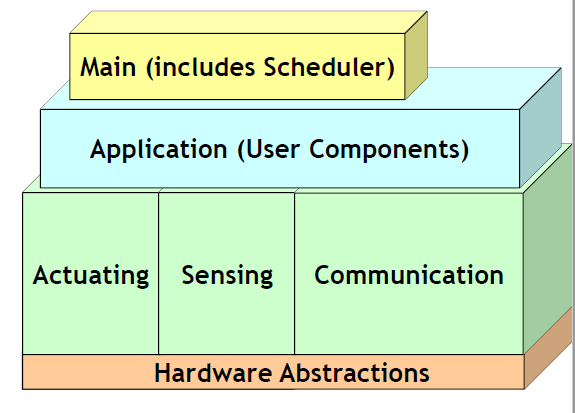
\includegraphics[height = 4cm]{TinyOS.png}
\end{center}
Besteht aus \textbf{Commands} (=Methoden), \textbf{Events} (Ereignisse), \textbf{Event-Handler} (kurze Funktion die beim Event abgearbetet wird), und \textbf{Task} (längere, asynchrone Funktion)
\begin{itemize}
	\item \textbf{Methode:} Aufruf \textsc{call}
	\item \textbf{Event:} (HW) Interrupt: \textsc{signal}
	\item \textbf{Tasks:} können alles
	\item \textbf{Scheduler:} FIFO
	\item Split-Phase-Operation: Event/command postet Task; wenn beendet, signalisiere Event
\end{itemize}
Zu den Komponenten gehören \textbf{Interface}, \textbf{Modul} (=Klasse), und \textbf{Configuration} (Komposition von Modulen, Anwendung). Darüber hinaus gibt es die Möglichkeit, Event-Handler aus der Ferne zu aktivieren (durch \textbf{Active Messages}). Eine AM enthält dabei die ID des Handlers und die Nutzdaten.
\subsection{Events: Freund oder Feind?}
Threads sind in der Regel bequem, aber oft ineffizient.\\
Events dagegen sind effizienter als Threads, aber oft umständlich.\\

Die Problematik bei Events ist, dass die Funktion aufgespalten werden muss. Dies führt zu
\begin{enumerate}
	\item globalen Variablen
	\item expliziten Zuständen
\end{enumerate}
\textbf{Verkettung} ist durch Aufruf des Events im Event möglich.
\subsection{OSM, andere}

\section{Vernetzung von Sensoren}
Es stellt sich die Frage, wie man einen Sensorknoten zum Netz verbindet.
\begin{itemize}
	\item \textbf{1-Hop:} Jeder Knoten kann mit jedem. Ausdehnung durch \textbf{Kommunikationsreichweite beschränkt}
	\item \textbf{Stern:} Alle Knoten mit leistungsfähiger Basisstation (zB SmartDust)
	\item \textbf{Cluster:} Sensorknoten kommunizieren \textbf{NUR} mit leistungsfähigem Head, Heads kommunizieren untereinander
	\item \textbf{Multi-Hop, Ad-Hoc:} Knoten kommunizieren mit Nachbarn, und nehmen andere als Knoten Router
\end{itemize}
Jeder Knoten kann zudem eine gewisse Knotenrolle annehmen. Zur Auswahl stehen dabei \textbf{Datenquellen} (Sensor), \textbf{Aggregatoren} (empfangen von mehreren Knoten, Reduktion), \textbf{Router} (leiten weiter) und \textbf{Senken} (Datenbank). Die Zuweisung ist dabei oft natürlich und hängt von der Netzstruktur ab.
\subsection{Senken}
Es sind Sammelstellen für Daten. Diese Stellen jedoch \textbf{Engpässe} dar, da Knoten in der Nähe der Senke viele Daten weiterleiten müssen (zB. EG Auswahl im Fahrstuhl).\\
Als Lösungsmöglichkeiten könnte man die Verwendung mehrerer Senken vorschlagen, oder eine erhöhte \textbf{Aggregation} der Daten im Netz.
\subsubsection{Sensor Internet}
Senken Könnten auch Gateways zum Internet bilden. Dadurch erhält man ein \textbf{globales} Sensornetz! \\
Hierfür sind aber weitere Schritte notwendig. Die Internet- und Web-Integration stellt eine große Herausforderung dar:
\begin{itemize}
	\item IP im Sensornetz? Oder soll das Protokoll übersetzt werden?
	\item IP-Adresse pro Knoten oder pro Netz?
	\item Wie repräsentiert man es als Web-Service?
\end{itemize}
\subsubsection{Sensor-Aktor-Netze} 
Bei Robotern oder Lampen gibt es neben Sensorknoten zusätzlich noch einen \textbf{Aktorknoten}. Diese werden mittels aus Sensordaten gewonnenen Informationen gesteuert. Hierbei gibt es \textbf{keine} Senken.\\

Im allgemeinen unterscheiden sich Netze aus Sensorknoten gerade dadurch. Bei Sensornetzen stehen die \textbf{Messdaten} im Vordergrund, nicht die Knoten. Die \textbf{Verarbeitung} der Daten geschieht im Netz, nicht an jedem Knoten selbst. Welcher Knoten Daten liefert ist grundsätzlich egal, da jeder Knoten identisch ist. Hierdurch wird die \textbf{Datenbasierte Adressierung} eingeführt: Man spricht mit allen Knoten, auf die eine Eigenschaft/Event zutrifft, nicht deren Adresse.\\

In WSN werden zudem die Protokollstacks verschmolzen. Dies wird als Hilfsmittel zur Optimierung von Energie- und Ressourcenverbrauch genutzt. Ein \textbf{gezielter Austausch} von Informationen wird somit ermöglicht.


	
	
	
	
	
	
	
	
	
	
	
	
	
	
	
	
	
	
	
	
	
	
	
	
	
	
\end{document}